% Chapter 2

\chapter{Matériels et méthode} % Main chapter title
\label{Chapter3} % For referencing the chapter elsewhere, use \ref{Chapter1}
%\minitoclt
\section{Zone d’étude}
\noindent{Pour mener notre étude, nous avons choisi la zone de production bananeraie de Toffo. Cette zone a été choisie, surtout, à cause de la diversité champs de bananier. On y retrouve d'autres cultures associées telles que le maïs, la canne à sucre, le niébé, le papayé, l'oranger... }

\noindent{La commune de Toffo concernée par notre étude est située dans la zone septentrionale du département  de l’atlantique avec une superficie de 492 $km^2$ environ $15\%$ de la superficie du département, et $0,42\%$ de la superficie totale du Bénin. Elle est limitée au Nord par la commune de Zogbodomey dans le département du Zou, au Sud par la commune d’Allada, à l’Est par la commune de Zè (au Sud-Est) et à l’Ouest par le fleuve Couffo servant de frontière naturelle avec la commune de Lalo dans le département du Couffo. La commune de Toffo est subdivisée en 10 arrondissements, décomposés en 54 villages. Le chef-lieu de la commune est  l’arrondissement de Toffo-centre situé à environ  81km de Cotonou (\cite{adjovi2006localisation}).}
\begin{figure}
	\centering
	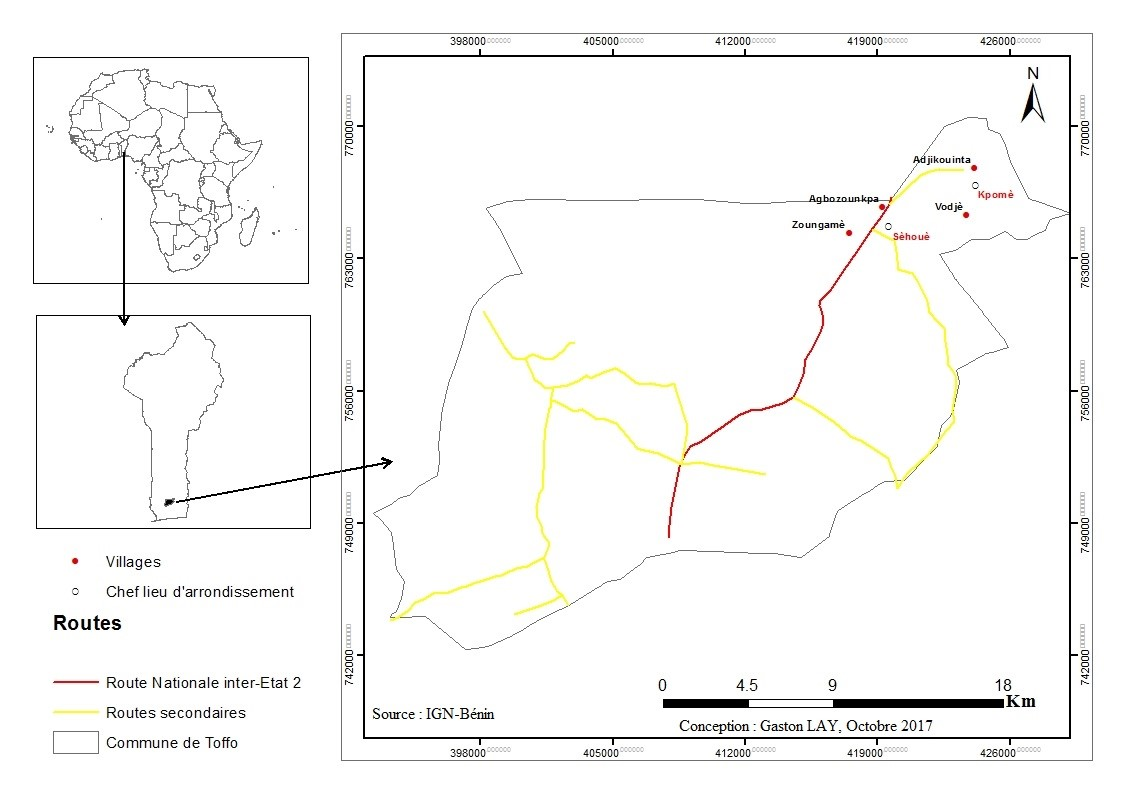
\includegraphics[scale=0.5]{carte}
	\captionof{figure}{Carte de la commune de Toffo}
\end{figure}
\section{Collecte des données}
\noindent{Nous utilisons dans ce travail comme données, les mesures de prédations journalières dans les champs de bananeraie de Toffo allant de 15 août au 5 septembre 2021. Ces données sont obtenues par protocole de proie sentinelle (\cite{ricci2017cartes}) }
\subsection{Protocole de « proie sentinelle » : }
\noindent{Le principe d’une proie sentinelle est d’exposer aux prédateurs des proies et de mesurer la proportion de proies consommées après un temps donné. Ici, nous utiliserions des charançons vivants que l’on entrave avec un petit fil de pêche, lui-même fixé au sol. La mesure consiste à noter la présence ou l’absence du charançon après 24h d’exposition. On dispose des petits morceaux de feuille de bananier pour offrir un abri au charançon, mais pas trop grand pour qu’ils restent exposés à certains moments (par exemple 4 morceaux de 4cm de côté).}
\begin{figure}
	\centering
	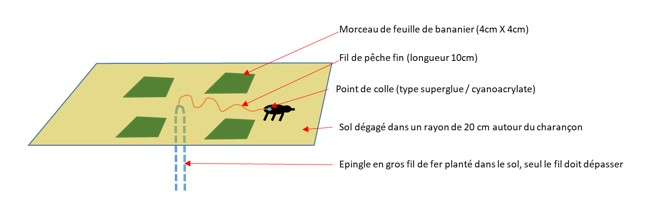
\includegraphics[]{proiesentinelle}
	\captionof{figure}{Protocole de proie sentinelle}
\end{figure}

\noindent{Une estimation du ratio de prédation peut être obtenue en confinant la proie et les prédateurs dans une cage placée au champ en conditions réelles. La limite de cette méthode est qu’elle ne donne pas d’indication sur la nature des prédateurs, elle ne donne qu’une estimation globale du ratio de prédation aux pieds des bananiers et des maïs, tous prédateurs confondus (\cite{mollot2012new}).}
\subsubsection{Méthodologie}
\noindent{Afin de simplifier l’approche, les cultures associées ont été restreintes à une culture la plus couramment rencontrée dans la zone étudiée (le maïs). Nous utilisons donc d’une approche par proies sentinelles afin d’estimer la prédation des adultes. La proie sentinelle a été déposée toujours à la même distance du bananier et de la plante associée. Nous procédons ensuite à la campagne de mesure de la prédation sur un réseau de parcelles avec à chaque fois la quantification de la prédation en zone proche des bananiers ou proche de la culture associée, en faisant à chaque fois des mesures appariées (bananier \& culture associée).\\
Vingt parcelles diversifiées (on observe la présence du maïs avec d'autres cultures telles que la canne à sucre, le niébé, le papayé, l'oranger...) ont été explorées avec cinq couples de charançons par parcelle. Les parcelles ont une longueur d’au moins 25m de côté afin de réaliser les mesures plus au centre pour limiter les effets de bord. La mesure dure 24 heures.
}
\begin{figure}
	\centering
	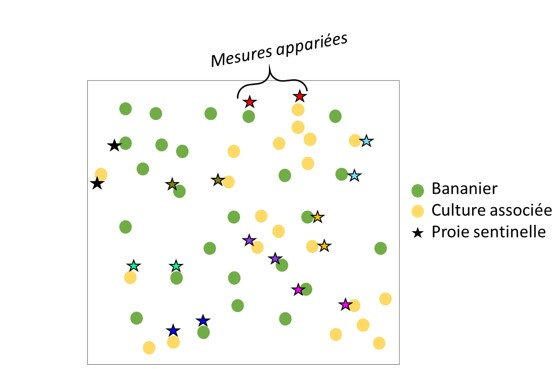
\includegraphics[]{placement}
	\captionof{figure}{Disposition de proie dans les champs}
\end{figure}
\begin{figure}
	\centering
	\includegraphics[height=15cm]{terrain}
	\captionof{figure}{ a)Photo de charançons attachés avant exposition dans le champ, b) Le charançon au début de son exposition dans le champ, c) Le champ d’exposition et d) Charançon consommé à 70\% après 24h  d’exposition dans le champ.}
\end{figure}

\section{Analyse statistique des taux de prédation de charançons dans un champ de bananier-maïs}
\noindent{Une base de données a été analysée  dans le but de s’informer sur le ratio de prédation entre les cultures de bananiers et maïs. Toute l’analyse statistique a été réalisée avec le logiciel \cite{rcitation}. Ce choix repose sur l’accessibilité du logiciel, ses mises à jours et l’accès à de nombreux packages  (utilisation notamment des packages lme4 \cite{lme4}, sjPlot \cite{sjplot} et emmeans \cite{emmeans}).}

\noindent{L’hypothèse d’indépendance des données n’étant pas vérifiée , le modèle choisit est donc le modèle linéaire mixte généralisé (GLMM ) (\cite{zuur2009mixed}). Ce modèle est une extension du modèle linéaire généralisé permettant la corrélation entre les observations et des données imbriquées.}

\noindent{Le seul effet aléatoire considéré est le champ. Nous ne cherchons pas à comprendre la prédation des charançons à l’échelle du paysage mais leur prédation dans de champ à petite échelle. Pour ce faire, nous utiliserons les groupes déterminés dans les champs, ce qui nous permettra de regrouper des états initiaux similaires. Le jeu de données tiré du protocole présente des données sur la régulation agro-écologie de 20 parcelles de culture de bananiers et maïs à Toffo. La prédation (Pred) a été mesurée pour cinq (5) couples de charançons sur chacune des 20 parcelles (champ) pour un total de 200 observations. La variable density mesure la densité de chaque parcelle en bananiers par rapport à la densité moyenne, tandis que la complexité de l'agro-écosystème est mesurée à l’échelle de la parcelle.
	
Les autres cultures souvent rencontrées sur les parcelles étant des tecks, papayés, orangers et palmeraies. La complexité agro-écologie a été calculée comme une variable de niveau qui exprime le nombre de cultures retrouvées dans la parcelle. La complexité est initialisée à 1 pour toutes les parcelles à cause de la présence du maïs. La complexité est donc la somme des variables binaires (absence ou présence des autres cultures sur une parcelle donnée)
	
Puisque la prédation représente la mort ou pas des charançons dans une parcelle, nous pouvons modéliser cette réponse par une régression binomiale, avec un effet fixe de la densité et un effet aléatoire du champ sur les deux coefficients. Le modèle suivant est appliquée sur nos données}

$logit(P_{ij})=\alpha + \beta_0*cult_{ij} + \beta_1*density_{ij}*complexite_i + \beta_2*champ_i$

\noindent{La notation logit correspondant au lien logistique (zuur2009mixed), $P_{ij}$ est la probabilité que le charançon j du champ i et de complexité i soit mort par prédation, $cult_i$ nous indique la plante hôte du charançon  (s'il s'agit d'un bananier ou du maïs), $complexité_i$ identifie la complexité agro-écologique et $champ_i$ identifie la parcelle. $density_{ij}$ est la densité de bananiers dans les champs.
	
La significativité des variables du modèle est testé en les supprimant à tour de rôle afin de comparer deux à deux le critère d'information d'Akaike (AIC) du modèle initial avec celui des sous-modèles. L’AIC mesure la qualité d’ajustement et la complexité du modèle (\cite{zuur2009mixed}) et est défini par l’équation suivante : $$AIC= -2\ln(L(\theta))+2K$$
avec $k$ le nombre de paramètres et $\theta$, la vraisemblance maximisée du modèle.\\
Pour chaque test réalisé, le seuil de significativité est de 0,05.	
}

\subsection{Résultats et discussion}
\begin{verbatim}
Single term deletions

Model:
pred ~ cult + density * complexity + (1 + density | champ)
				   npar    AIC    LRT  Pr(Chi)   
<none>                  274.01                   
cult                  1 279.88 7.8719 0.005021 **
density:complexity    2 270.03 0.0214 0.989347   
---
Signif. codes:  0 ‘***’ 0.001 ‘**’ 0.01 ‘*’ 0.05 ‘.’ 0.1 ‘ ’ 1
\end{verbatim}
\noindent{L'AIC pour le modèle dans lequel aucun terme n'est supprimé est de 274.01. En supprimant la variable nominale cult (culture) de ce modèle, l'écart augmente à 279.88, soit une variation de 5.87. La variation de déviance pour le GLM binomial est distribuée par un chi carré avec 1 degré de liberté et a une p-value inférieure à 0,01, ce qui signifie que le terme est  significatif. En supprimant le terme d'interaction seul, on observe une réduction de 3.98 de l'AIC et qui n'est pas significatif. \\
	Pour avoir une idée de ce que fait le modèle, nous avons voulu visualiser les valeurs prédites.}
\begin{figure}
	\centering
	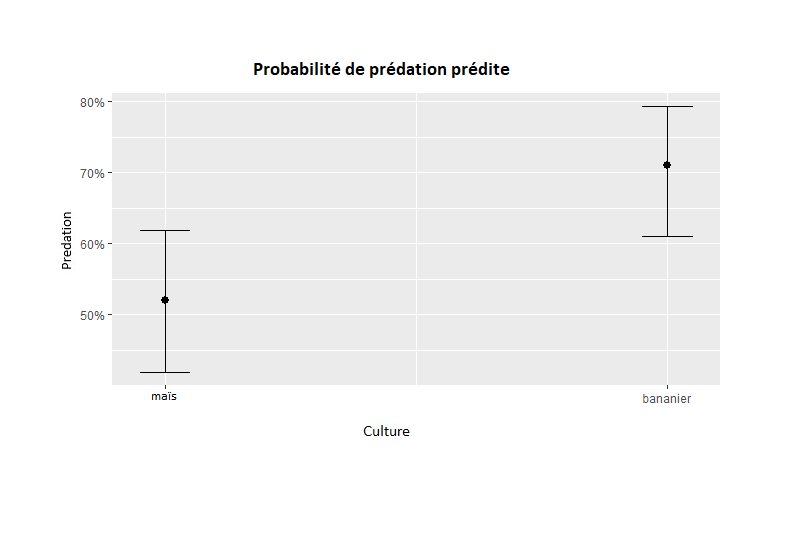
\includegraphics[height=12cm]{ratio}
	\captionof{figure}{\label{rat}Taux de prédation des charançons aux pieds des bananiers et des maïs dans les champs.}
\end{figure}

\noindent{la figure \ref{rat} nous informe sur le taux de prédation des ravageurs aux pieds des bananiers et des maïs. La moyenne aux pieds des maïs est d'environ 52\% et 71\% pour le bananier. L’exposition de proies sentinelles est une technique relativement biaisée par rapport à la prédation naturelle de ravageurs (proies mortes, messages d’odeurs agrégation ou surexposition plus ou moins volontaire des proies) \cite{ricci2017cartes}. Ceci nous amène à considérer un rapport de prédation entre le taux de prédation au pieds des bananiers et des maïs et ceci sur une durée de vie des charançons. Nous considérons donc un ratio de 52/71}

\begin{figure}
	\centering
	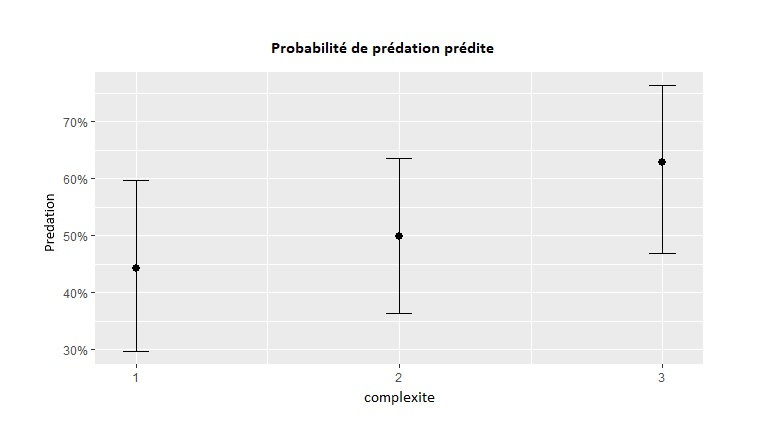
\includegraphics[height=10cm]{complexite}
	\captionof{figure}{\label{complec}Taux de prédation prédit par GLMM en fonction de la complexité  des champs.}
\end{figure}

\noindent{De ce graphique, on retient que dans les champs de bananiers et maïs uniquement (complexité = 1), il y a un taux moyen d’environ 0.45 de prédation pour un charançon donné (ce taux peut varier entre 0.3 et 0.6). Le taux moyen augmente au fur et à mesure que la diversité des parcelles devienne plus complexe. Tout ceci conforte l’hypothèse d’une régulation de charançons importante dans les champs avec les cultures associées (diversité agro-écologique complexe). Östman et al., (2001) et de Chaplin-Kramer et al., (2011) font ressortir que dans la plupart des situations, les paysages plus complexes, comportant davantage d’habitats semi-naturels, sont associés à une plus grande abondance et à une plus grande diversité d’ennemis naturels, ce qui augmente donc la probabilité de prédation des ravageurs.
}
\begin{figure}
	\centering
	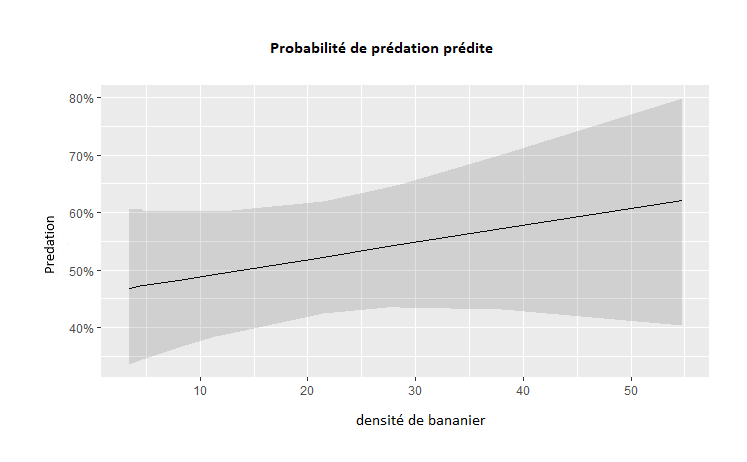
\includegraphics[height=10cm]{densite}
	\captionof{figure}{\label{dens}Taux de prédation prédite par GLMM en fonction de la densité bananiers dans les champs.}
\end{figure}
\noindent{La figure \ref{dens} nous montre le taux de prédation des ravageurs en fonction de la densité de bananiers dans les champs. On constate une tendance de moyenne linéaire qui croit avec la densité. En effet, la lutte par les ennemis n'est efficace qu'en présence d'une forte densité des ravageurs (\cite{gold2000biology}). On fait donc l'hypothèse que plus le champ est dense, plus on est susceptible d'avoir une forte densité de ravageurs aussi. Optimal foraging theory suppose que le prédateur cherche à obtenir le plus de ressources tout en minimisant le temps passé à chercher sa proie (\cite{davies2012introduction}). L’évolution des prédateurs vers le spécialisme ou le généralisme peut donc dépendre de la quantité de proies disponible. L’optimal foraging prédit que lorsque la ressource optimale est abondante, les prédateurs ont tendance à se spécialiser sur cette ressource, car ils perdent peu d’énergie à chercher leur proie optimale (\cite{davies2012introduction}).}

\subsection{Conclusion }
\noindent{Dans le but de lutter contre les ravageurs, la complexité de l’agrosystème s’est avérée comme un bon moyen de régulation naturelle. De plus, ces qualités en tant qu’un service de régulation biologique ont déjà été appréciées dans d’autres études. Nous nous basons donc, sur le ratio de prédation pour proposer un modèle mécaniste simulant la prédation des \textit{C. sordidus}. pour différentes configurations d'association de culture de bananier avec le maïs.}

\section{Modèle mécaniste COSMOSPARK}
\noindent{Le modèle vise à simuler les pratiques agricoles et son environnement animal et végétal dans le but de prédire l’évolution des populations de bioagresseurs et d’éviter leur installation. Nous nous sommes intéressés ici aux bananeraies intercalé avec le maïs et à leur ravageur principal, le charançon \textit{Cosmopolites sordidus}. Le modèle Cosmospark basé sur les individus a été implémenté dans NetLogo (\cite{tisue2004netlogo}), et sa description est détaillée en utilisant le protocole ODD (\cite{grimm2010odd} ; \cite{grimm2013individual})}
\subsection{Description et paramétrage du modèle}
\noindent{Le modèle est basé sur des données de présence-absence de charançons dans un ensemble d'habitats. Ces données instantanées sont collectées sur une seule génération (les adultes) et sont supposées représenter le quasi-équilibre de la dynamique des métapopulations. L'objectif de la modélisation est d'ajuster la fonction d'incidence aux données instantanées observées, afin d'obtenir des estimateurs des paramètres du processus spécifique aux\textit{C. sordidus}. Une fois ces paramètres connus, le modèle peut être utilisé pour prédire les probabilités de prédation spécifiques à l'habitat pour une configuration particulière de l'habitat. Ainsi, les taux de prédation peuvent-être prédits pour chaque type d’habitat. Cette prédation est supposée se produire au hasard pour chaque habitat.
	
\begin{table}
	\small
	\caption{\label{parametre}Paramètres du modèle. Ces paramètres proviennent du modèle de base. Nous ajoutons ici, le taux de prédation au pied de bananier. }
	\begin{tabular}{L{5cm} @{} C{1.5cm} @{} C{1.5cm} @{} C{5cm} @{} L{3cm} }
		\hline Description & Code & Valeur &Intervalle utilisé pour l’analyse de la sensitivité & références\\
		\hline \textbf{Adult} & & & &\\
		Sex-ratio (male:female) & -- & 1:1 & -- & \cite{gold2001biology}\\
		Sexual maturity for females after
		emergence (days) & SM & 34.5 & 33-36 & \cite{cuille1950recherches}\\
		Probability of egg-laying on 
		maiden sucker compared to flowered plants & OMPS & 0.11 & 0.08-0.13 & \cite{abera1997oviposition}\\
		Probability of egg-laying on
		preflowered plants compared to
		flowered plants & OPPF & 0.41 & 0.39-0.46 & \cite{abera1997oviposition}\\
		Number of adults per week
		necessary for density-dependent effect
		on fecundity & DE & 20 & 10-33 & \cite{abera1997oviposition}\\
		Number of eggs per week per female
		without density-dependent effect & FH & 2.7 & 1.7-3.2 & \cite{koppenhofer1993observations}\\
		Number of eggs per week per female
		with density-dependent effect & FL & 0.8 & 0.6-1.1 & \cite{abera1997oviposition}\\
		Maximum lifespan of adult (days) & ML & 748 & 542-748 & \cite{froggatt1926banana}\\
		Proportion of individuals moving 2 m
		per time step (\%) & DC1 & 1.4 & 1.5-6.6 & \cite{delatre1980insect}\\
		Proportion of individuals moving 4 m
		per time step (\%) & DC2 & 0.3 & 0.0-3.0 & \cite{delatre1980insect}\\ 
		& & & & \\
		\textbf{Banana plant} & & & & \\
		Banana maize predation & BMP & 0.03 & 0.02-0.2 & --\\
		Interval planting–maiden sucker
		(degree-days) & -- & 800 & -- & \cite{abera1997oviposition}\\
		Interval planting–preflowering
		(degree-days) & -- & 1600 & -- & \cite{abera1997oviposition}\\
		Interval planting–post-flowering
		(degree-days) & -- & 2350 & -- & \cite{tixier2004simba}\\ 
		\hline 
	\end{tabular}
\end{table}
}


\subsection{Caractéristiques générales du modèle COSMOSPARK}
\noindent{Le modèle COSMOSPARK est un IBM stochastique qui fonctionne sur un pas de temps quotidien. C’est une extension du modèle COSMOS (\cite{vinatier2009cosmos}) simulant le mouvement local et la ponte des femelles dans le champ, l'infestation des larves dans les bananiers, et les principales caractéristiques du développement de l'insecte et de la plante hôte. COSMOSPAK intègre à cet effet la prédation des charançons adultes en ajoutant une culture favorable à la prédation (le maïs). Selon le modèle, les individus \textit{C. sordidus} se dispersent dans un champ représenté par une grille avec un bananier par cellule (la surface de la grille varie entre 144 et 441 m2). Les plantes de bananiers passent par trois étapes distinctes jusqu'à la récolte : le drageonnage, la préfloraison et la post-floraison. Juste avant la floraison, on sélectionne un nouveau drageon de la plante mère qui pousse simultanément dans la même cellule. Le délai entre deux récoltes consécutives, correspondant à un cycle de culture, est d'environ 200 jours (voir \cite{tixier2004simba} pour des détails sur les cycles de culture du bananier). Les femelles de \textit{C. sordidus} pondent des œufs sur les bananiers, et les larves issues de ces œufs percent le cornet des plantes. La durée des stades des juvéniles et les stades phrénologiques des bananiers dépendent de la température. Les plantes de maïs sont considérées comme statique dans le modèle faisant apparaitre une mortalité par prédation. Les prédateurs ont été caractérisés par un "effet prédation" distribué sur les cellules de plantes en fonction de la proximité de maïs. La figure \ref{uml} présente le modèle et ses caractéristiques. }
\begin{figure}
	\centering
	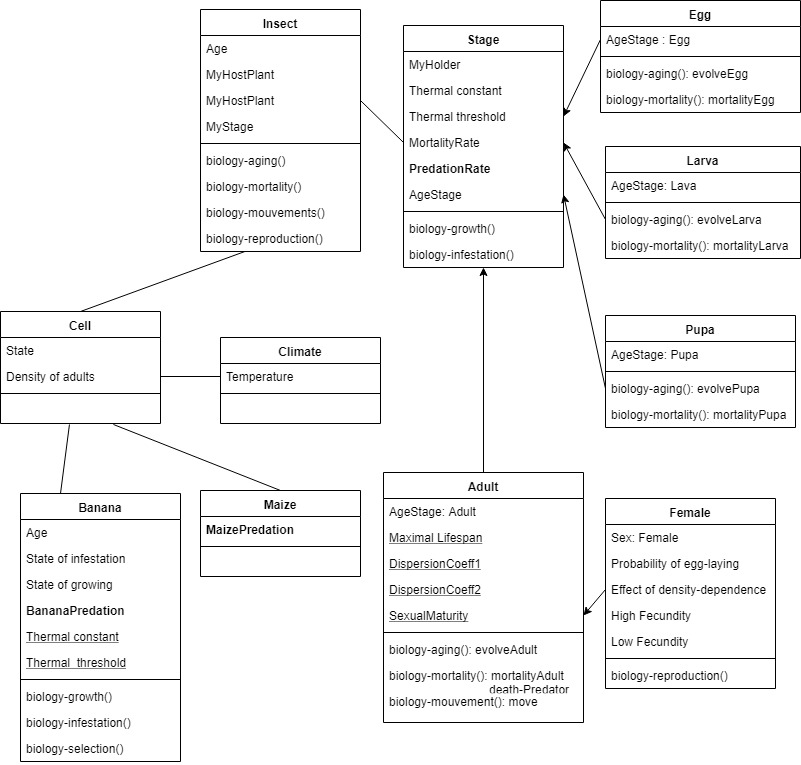
\includegraphics[height=15cm]{UML_COSMOSPARK}
	\captionof{figure}{\label{uml} Diagramme de classes du modèle COSMOSPARK.}
\end{figure}

\subsection{Protocole ODD}
\subsubsection{Overview}
\subsubsection{Purpose}
\noindent{Le but de notre modèle est de simuler la prédation de \textit{C. sordidus} par les arthropodes prédateurs en décrivant comment des patterns d’organisation spatiale (bananiers \& culture associées) modifient la dynamique des populations de charançon sur une parcelle donnée.}
\subsubsection{Entities, state variables and scales}
\noindent{Le modèle COSMOSPARK comporte 3 entités, les charançons, les bananiers, les maïs. Les charançons sont décrits par 3 variables d’état : l’emplacement –x, y – leur stade de vie et leur sexe. Les bananiers sont décrits par leur emplacement (cellule de grille) et une liste numérique contenant le taux de mortalité journalier sur chaque bananier en fonction de sa configuration. Les maïs aussi sont décrits par leur emplacement (cellule de grille) et une liste numérique contenant le taux de mortalité journalier fixe sur chaque maïs. Les unités spatiales sont caractérisées par leur emplacement (cellule de grille) et leur type d'habitat. Les deux types d’habitats sont les habitats de culture contenant bananiers et maïs (habitat favorable aux prédateurs).  L’habitat proche de culture de maïs est considéré comme favorable à la régulation des charançons et donc a d’effet sur les charançons.Les parcelles de champ de bananiers- maïs dans le modèle sont de 25 m x 25 m et ont un grain de 2 x 2 m. La superficie de la parcelle a été choisie pour faciliter la prise en compte de divers modèles spatiaux de cultures et d'un nombre et d'une densité raisonnables de plants de bananes (1736 plants de bananes /ha ; Vinatier et al, 2009). Une parcelle est alors une grille carrée de 50 x 48 cellules traitée comme un tore. Tous les bananiers et les mais sont placés sur des cellules côte-à-côte les uns des autres pour limiter l’effet du sol nu.
Les charançons ont une durée de vie en moyenne de deux ans. Le modèle fonctionne sur un pas de temps journalier pendant deux ans donc, 748 jours.}
\begin{figure}
	\centering
	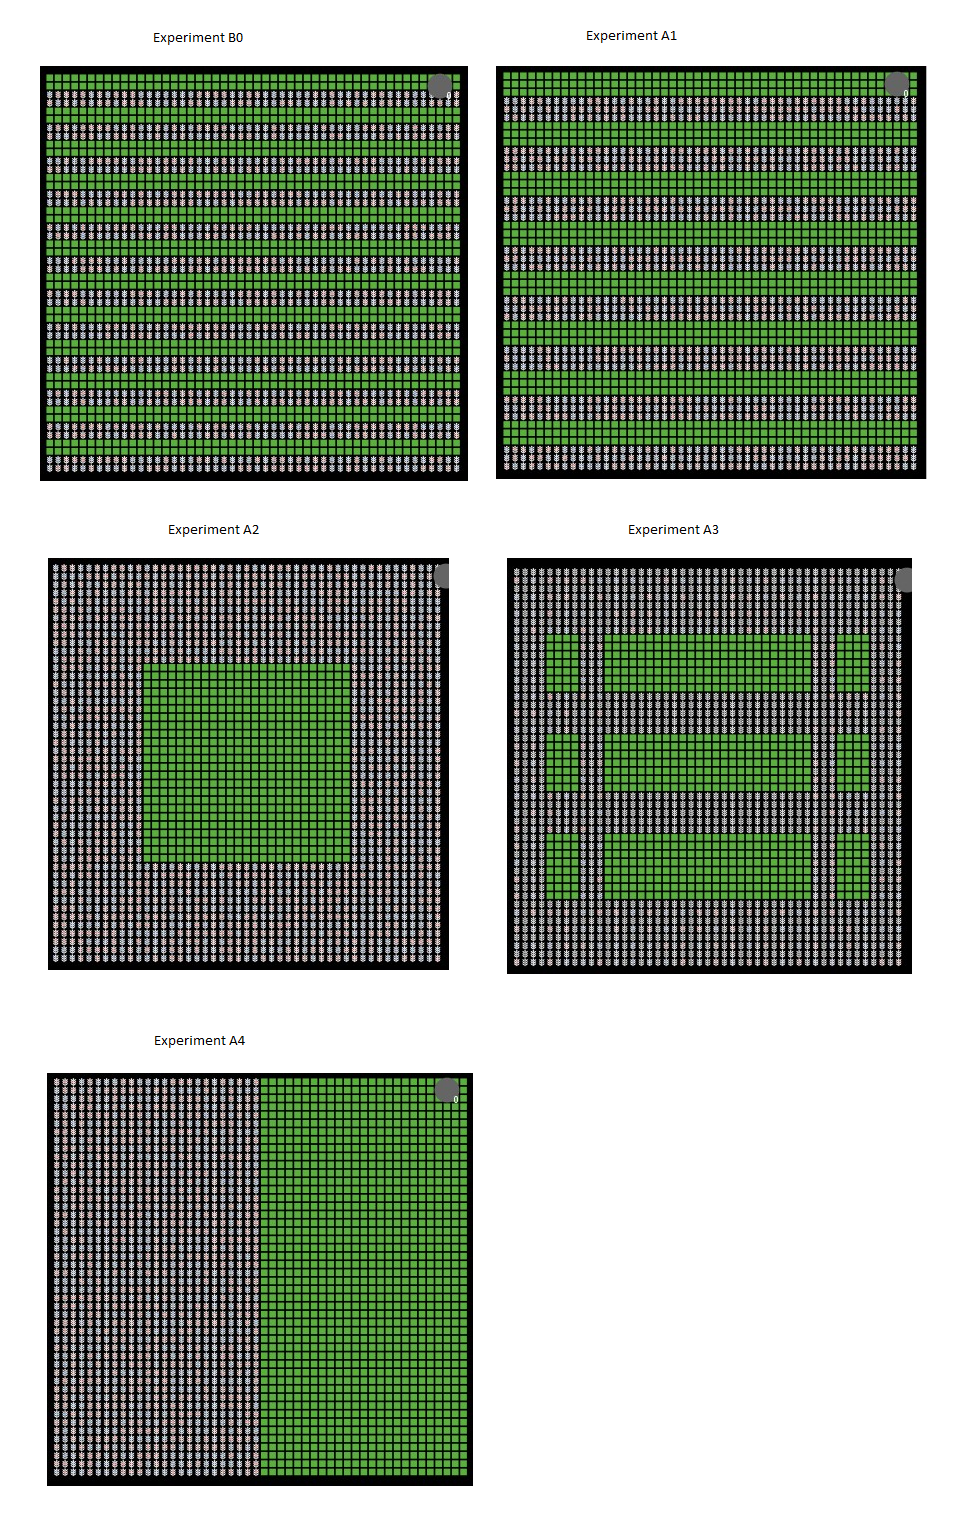
\includegraphics[width=12cm]{Patterns}
	\captionof{figure}{\label{patterns} Les patterns du modèle. Les bananiers sont en blanc et les maïs en vert. Les charançons ont été disposés aux pieds de bananiers.}
\end{figure}

\subsubsection{Process overview and scheduling}
\noindent{Les processus de simulation du modèle sont décrits dans l'organigramme (Fig. \ref{flowchaart}). A chaque pas de temps, deux sous-modèles sont exécutés dans l'ordre suivant : La prédation et l'observation des bananiers. La prédation est exécutée pour tous les ravageurs dans un ordre aléatoire et défini le fait qu'ils soient tués ou pas en fonction de la configuration du champ. Le sous-modèle Observation des bananiers est ensuite exécuté pour tous les bananiers dans un ordre aléatoire et enregistre le nombre de ravageurs présents dans la parcelle.}
\begin{figure}
	\centering
	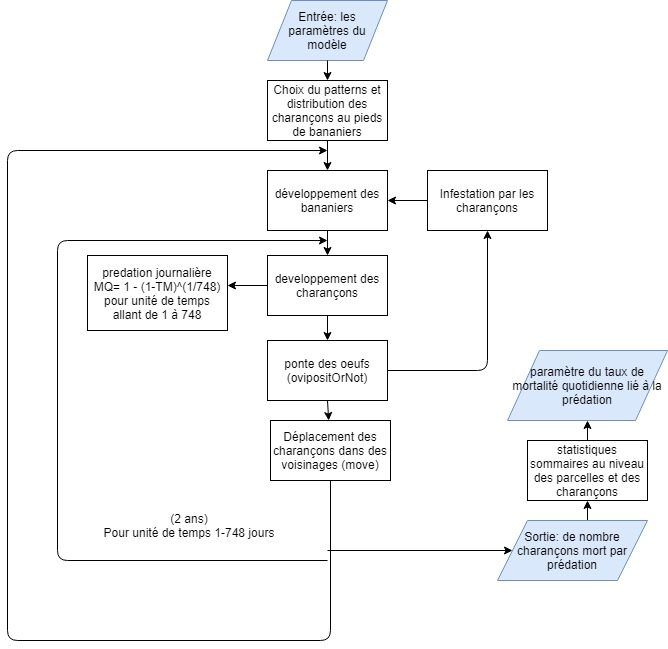
\includegraphics[width=12cm]{flowchart}
	\captionof{figure}{\label{flowchaart} Organigramme du modèle de simulation examinant la relation entre l’organisation des parcelles et le taux de prédation.}
\end{figure}
\subsubsection{Design concepts}
\noindent{\textit{Basic principles :} Le modèle est une extension du modèle COSMOS qui simule l'épidémiologie spatiale de \textit{C. sordidus} à long terme en décrivant la dynamique de sa population et l'infestation des plantes hôtes qui en résulte. L’ajout des maïs au modèle constitue un habitat favorable aux prédateurs généralistes dont l’effet a été modélisé par la fixation des taux, sur des patches, qui varient en fonction du type d’habitat.

\textit{Emergence :} La dynamique des mouvements des charançons et la pression de prédation qui en résulte sur l'ensemble des bananiers émergent du comportement de recherche de nourriture des individus. L'interaction entre les mouvements, l'effet dilution et l'organisation spatiale n'est pas simple.

\textit{Adaptation :} agents purement réactifs

\textit{Objectives :} agents purement réactifs

\textit{Learning :} agents purement réactifs

\textit{Prediction :} agents purement réactifs

\textit{Sensing :} Les bananiers sont sensible au climat. Les charançons ne peuvent percevoir que l'habitat où ils se trouvent au début de l'étape de temps et les habitats qu'ils traversent au cours de leurs déplacements aléatoires.

\textit{Stochasticity :} Dans le modèle, la construction des parcelles (simulation des parcelles), les mouvements individuels et les décisions de prédation sont stochastiques. Les mouvements sont classiquement modélisés par une chaîne de Markov de premier ordre. Par conséquent, la stochasticité a également été choisie pour les décisions des ravageurs de bouger.

\textit{Observation :} Pour une simulation (748 jours), les listes numériques des ravageurs sont importées de Netlogo vers R (\cite{rcitation}) via le package RNetlogo (\cite{thiele2014r}; \cite{thiele2012rnetlogo}). Les statistiques sommaires du nombre de ravageurs mort par prédation tenant compte de l’organisation spatiale ont été calculées via R (voir la définition détaillée des paramètres dans le tableau \ref{parametre}). Nous observons donc, la moyenne des infestations et la proportion de plantes sévèrement infectées en fonction des patterns.

\textit{Collectives :} Il n’y a pas de collectif mais, il y a une densité des charançons qui influe sur leur capacité à se reproduire.
}
\subsubsection{Details}
\noindent{\textit{Initialisation :} Le modèle est initialisé en assignant des types d'habitats aux cellules (c'est-à-dire des simulations de parcelles), en spécifiant les paramètres prédation et en distribuant les ravageurs aux pieds des bananiers dans une parcelle.
	
\textit{Input data :} Il n’y a pas de données externes dans notre modèle mis à part les paramètres du modèle.
}

\subsubsection{Submodels}
 \noindent{ \textit{Move :} Le déplacement des  charançons est influencé par l’habitat dans lequel il se trouve. Les animaux utilisent une grande variété d'indices chimiques, visuels et acoustiques pour évaluer l'aptitude de l'habitat à fournir de la nourriture (\cite{searle2005should}), la ponte (\cite{rabasa2005egg}) ou la protection contre les prédateurs (\cite{hufker1999az}). La perception d’habitat par un individu est définie par le noyau de dispersion qui prend compte des contraintes de déplacement d’un habitat à un autre en fonction de la distance par rapport à l’emplacement actuel. Bien qu’ils soient considérés comme statique dans le temps et dans l’espace (\cite{chapman2007modelling} ; \cite{coombs2007field}), les noyaux de dispersion peuvent différer en fonction du temps (\cite{phillips2008reid}), de facteurs intrinsèques tels que le sexe, l'âge, le statut social ou les réserves énergétiques, et des conditions environnementales telles que le climat, la saison, la qualité de l'habitat, la compétition, la prédation et le parasitisme (\cite{bianchi2009foraging}; \cite{walters2006modelling}). En se servant des récentes avancées en matière de radiopistage des individus (\cite{schick2008understanding}), et en considérant le mouvement individuel des charançons comme une marche aléatoire dans laquelle les lieux d'arrivée et de départ des individus dépendent des caractéristiques de l'habitat et de leur distance par rapport à l'emplacement actuel de l'individu, (\cite{vinatier2010radiotelemetry}) ont défini la probabilité de déplacement d'une cellule a à une cellule b de la grille dans une unité temporelle par une chaîne de Markov de premier ordre définie par :
 $$Pr(a \rightarrow b)=\frac{\alpha_{h(b)}f_{\beta h}(d_{ab})}{\sum_{k=1}^{m}\alpha_h(k)f_{\beta h}()d_{ak}}$$

Où $\alpha_{(h(k))}$est la préférence relative pour l'habitat $h$ de la cellule $k$, $d_{ak}$ la distance entre les cellules $a$ et $k$ et $f(d_{ak})$ le noyau de dispersion dépendant de la distance définie par $exp^{((-\beta a.d_{ab}))}$ La décision individuelle de se déplacer a été basée sur une probabilité multinomiale entre toutes les probabilités calculées sur la grille. Pour l'efficacité du calcul, les cellules avec des probabilités proches de zéro n'ont pas été considérées dans la probabilité multinomiale.

\textit{Death-predator :} La mortalité due à la prédation est journalière et suit une distribution binomiale avec une probabilité dépendant de la configuration spatiale et du type d’habitat sur lequel se retrouve le charançon. Dans un champ de bananier avec maïs intercalé, le taux de prédation est censé suivre une distribution de poisson (\cite{hilker2006parameterizing}). Si le charançon se trouve sur un habitat bananier avec un l’habitat maïs situé à une distance de prédation (d) donnée, le charançon a une probabilité : $$p=1-(1-MQ)^{(\frac{1}{ML})} $$ d'être bouffé \cite{bousquet2001multiagent}.

Avec $MQ$ : la mortalité quotidienne et $ML$ : la durée de vie d’un charançon }
\subsection{Procédure de simulation}
\subsubsection{Validation du modèle}
\noindent{La simulation a été réalisée dans une zone de 52*52 cellules (dimension de cellules 2,4 *2,4). Chaque bananier appartenait à une cellule ainsi que chaque maïs. Le modèle a été rendu simple en ne laissant aucune cellule vide donc toutes cellules contenaient chacune un bananier ou maïs. Les simulations ont été effectuées sur 748 jours, correspondant à la durée de vie d’un charançon. Pour l’estimation du taux quotidien de mortalité, nous avons, dans un premier temps établi une relation pour calculer le ratio de régulation de la population de charançons aux pieds des bananiers et des maïs en utilisant les données obtenues par proie sentinelle dans les champs de bananeraies de Toffo. Le ratio de régulation de \textit{C. sordidus} était 52/71 dans un champ de bananiers avec maïs intercalé. Le taux de mortalité quotidien a été ensuite varié entre 0 et 1 sur les différents patterns (fig. \ref{patterns}). En analysant la figure, on constate qu’à partir de 0.2, on obtient  presque une croissance de charançons qui est quasi-nulle pour les cinq patterns.}
\begin{figure}
	\centering
	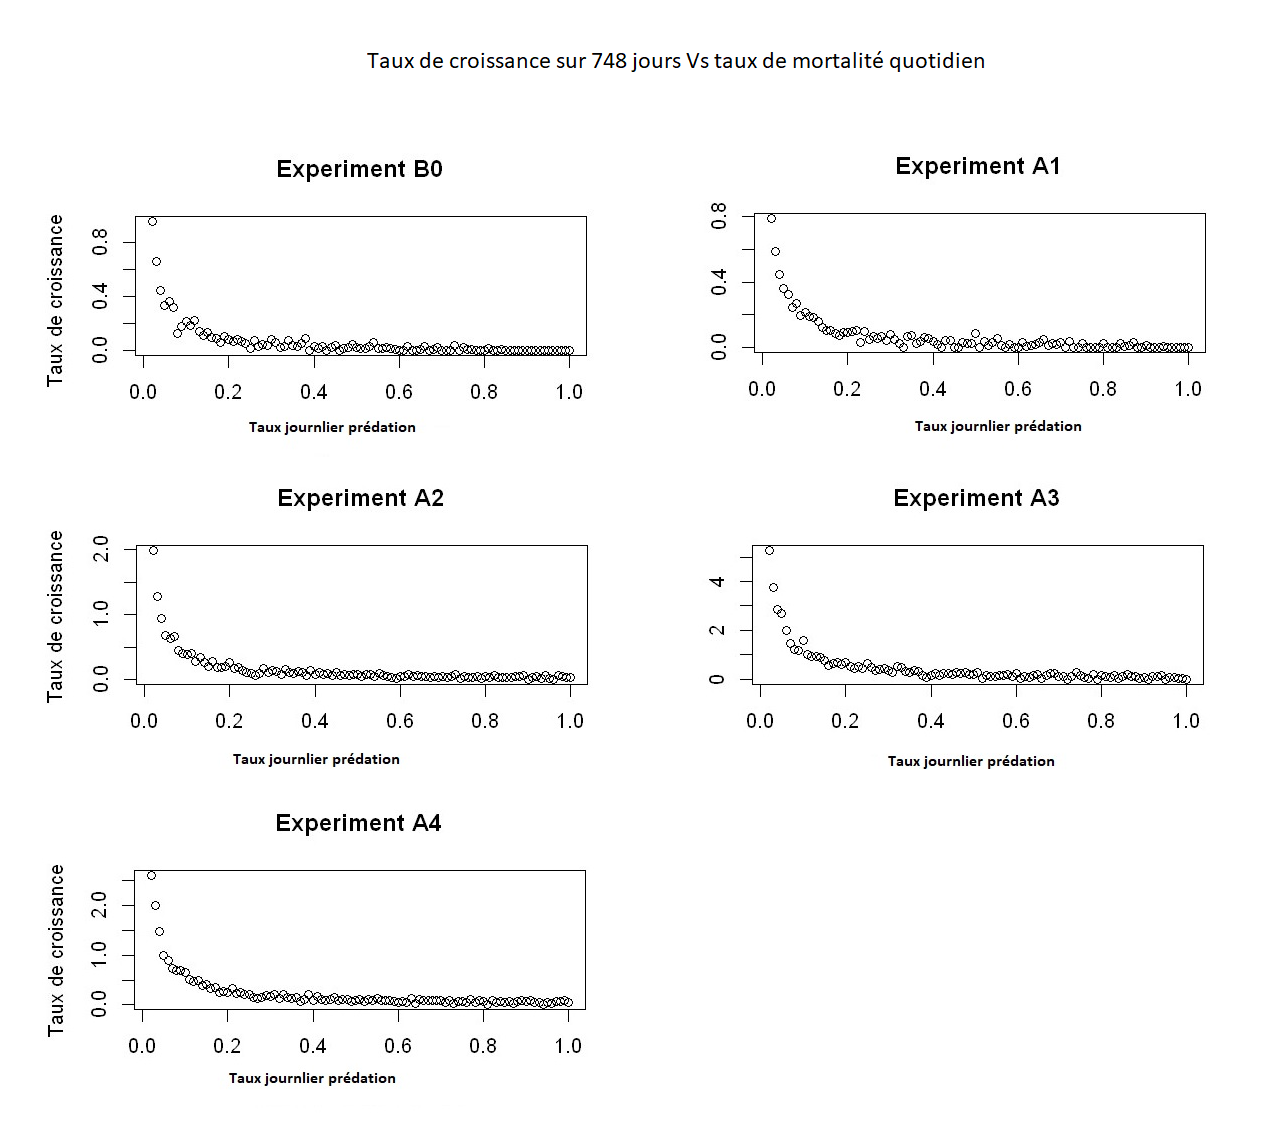
\includegraphics[width=17cm]{rate}
	\captionof{figure}{\label{taux} Recherche d'une approximation du taux de mortalité quotidien.}
\end{figure}
\noindent{En raison de la stochasticité du modèle, nous avons donc effectué 20 répétitions pour chaque situation en restreignant l’intervalle du taux quotidien de mortalité à un intervalle compris entre 0 et 0,2   et avons calculé la moyenne des résultats (fig. \ref{tauxcrs}).}
\begin{figure}
	\centering
	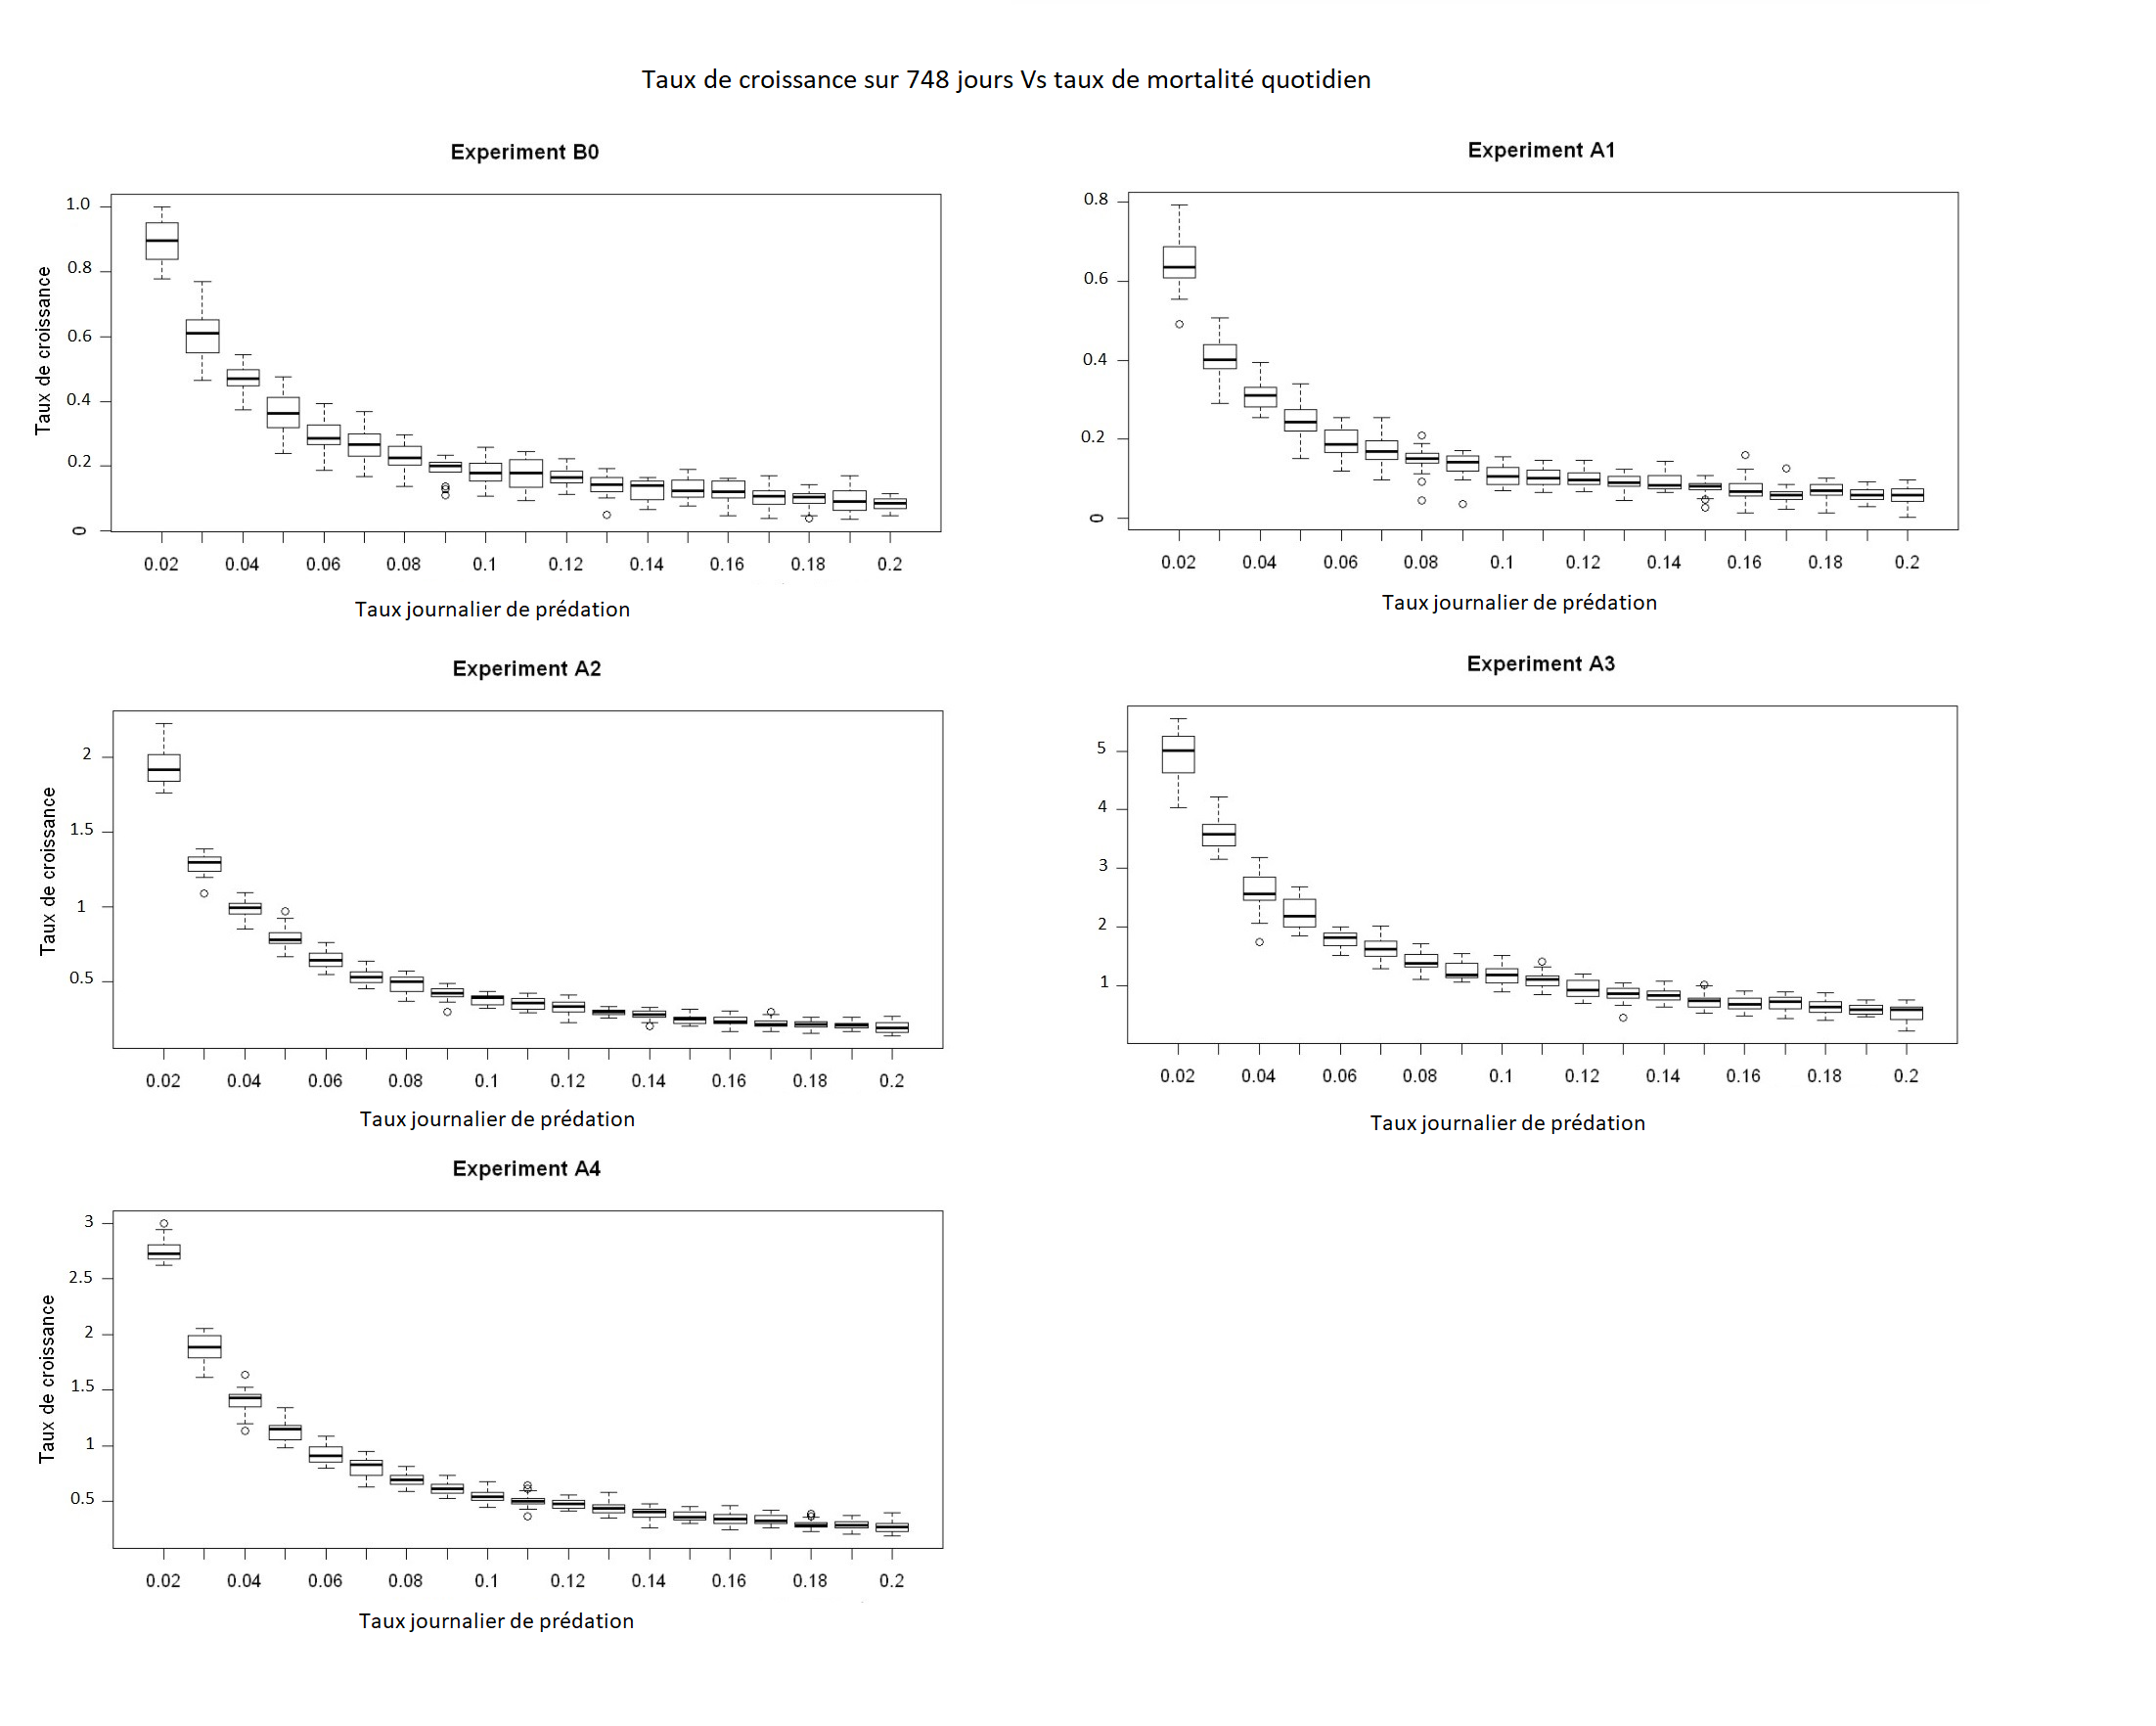
\includegraphics[width=17cm]{tauxcroissance}
	\captionof{figure}{\label{tauxcrs} Analyse de la sensibilité du modèle COSMOS aux paramètres écologiques des parcelles  les plus influents, en se concentrant sur le  paramètre principal de la distribution des taux moyens de régulation quotidienne  sur la parcelle d’expérience B0. Une gamme de valeurs a été testée pour le paramètre, les autres paramètres étant maintenus constants. Le résultat de 20 exécutions a été calculé dans un boxplot.}
\end{figure}
\noindent{Sous l'hypoyhèse des taux de prédation pouvant aller jusqu'à 70 \% (\cite{perfecto1998deployment}) au bout de deux ans dans des champs diversifiés, il a été choisi, en se basant sur les boxplot, comme taux de prédation quotidien 0.03}
\subsubsection{Résultat}
\noindent{La croissance de la population des ravageurs a été affectée par l'organisation spatiale dans leur environnement proche (Fig. \ref{patterns}). Cependant, les effets de l'organisation spatiale diffèrent selon la durée de vie des charançons. On observe une réduction subite de la population des charançons (0,2 ±  0,1) entre le 1er et le 100ième jour pour les patterns d’expérience (ExperimentB0 et ExpérimentA1). La population croit après les 100 jours mais est régulée par l’activité favorable des cultures associées. Par contre pour les patterns d’expérience ExperimentA2, ExperimentA3 et ExperimentA4 (Fig. \ref{patterns}) la population connait une même baisse entre les 100 premiers jours mais croit de manière presque linéaire après jusqu’aux 748ème jours. Comme résultat, la configuration spatiale (ExperimentB0 et ExperimentA1) où les plantes de bananiers sont intercalées avec les plantes de maïs favorise une meilleure gestion de ravageurs par des prédateurs généralistes. La régulation observée durant les 100 premier jours pour toutes les configuration est due à la densité des ravageurs au début du modèle, ce qui favorise l'efficacité de l'activité des ravageurs (\cite{davies2012introduction}).}

\begin{figure}
	\centering
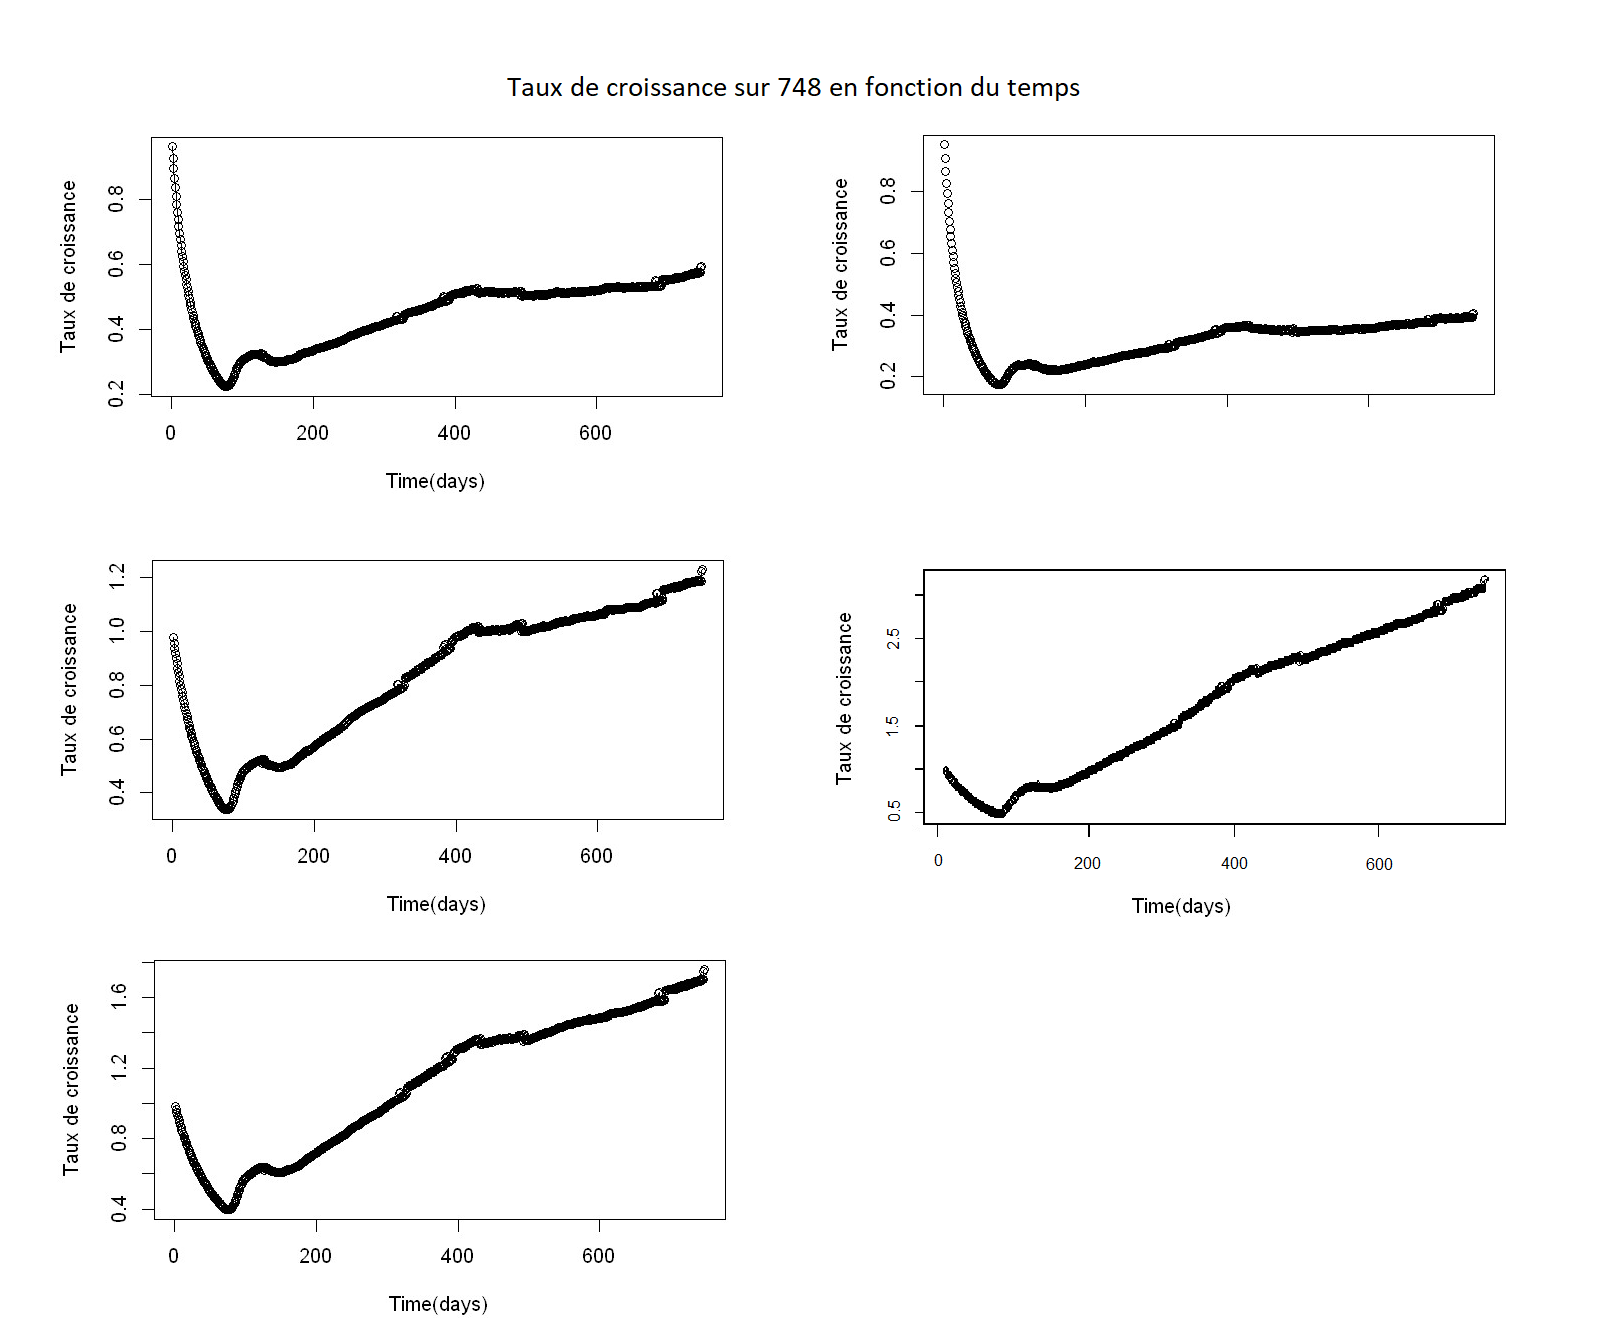
\includegraphics[width=17cm]{croissancetemps}
\captionof{figure}{\label{tauxcrs} Simulation de la distribution du taux de croissance des ravageurs en fonction du temps.}
\end{figure}

\subsubsection{Discussion}
\noindent{En partant d'un modèle spatialement explicite pour une prédation dans des champs de bananiers avec cultures associées, nous avons montré que le taux de croissance de la population des ravageurs peut-être affecté par la configuration spatiale de la parcelle. En ne prenant pas en compte l’intervalle de plantation des cultures, le cycle de maïs  et la mobilité des prédateurs, ce modèle nous a permis de mieux comprendre la régulation des ravageurs causée par la présence des cultures associées (maïs).

Le modèle omet certains comportements ou interactions complexes, tels que le mouvement du prédateur dépendant de la densité ou la capacité du prédateur à évaluer la qualité de l'habitat à distance, qui pourraient influencer la recherche de nourriture, le cycle de maïs qui varie selon le temps et qui pourrait ralenti la régulation pendant la récolte,  Ces omissions peuvent donc réduire le pouvoir prédictif du modèle. Néanmoins, le modèle est une première étape et peut être modifié à l'avenir par l'ajout de complexité en fonction de l'espèce et du système considérés.

Notre modèle ne représente pas les prédateurs ou le cycle des maïs. Cependant, l'inclusion des prédateurs généralistes nécessite généralement des hypothèses concernant la dynamique des prédateurs et les interactions avec les ravageurs, ce qui peut rendre les résultats moins généralisables ou conduire à une propagation des erreurs si les hypothèses sont inexactes. Ceci suggère donc une question qui est de savoir s'il est toujours pertinent d'utiliser la modélisation multi-agent à des questions agroécologiques, à cause de la complexité des systèmes de cultures. Dans l'étude actuelle, l'effet potentiel des prédateurs sur les ravageurs a été évalué par l’hypothèse de distribution des taux de prédation aux pieds des plantes en fonction du voisinage d’habitat favorable. Ces mesures pourraient être plus améliorées en réalisant des mesures journalières sur une durée de 3 mois minimum avec des méthodes de technologie avancée (observation avec caméra ou par image) et intégrant le cycle de maïs  selon la température. }

\subsubsection{Conclusion}
\noindent{Les résultats de la présente étude démontrent que la diversité des cultures affecte fortement le contrôle biologique des ravageurs. Nous avons constaté que l’effet des prédateurs par parcelle est fortement affecté par la configuration spatiale. Dans l'ensemble, nos résultats suggèrent que l'organisation spatiale des cultures associées est un outil qui peut être utilisé par les agriculteurs pour améliorer la lutte biologique des ravageurs. Cependant, les effets secondaires doivent être pris en compte avant que les agriculteurs ne soient invités à mettre en œuvre une organisation spatiale donnée, comme la capacité d'un prédateur spécifique à éliminer les parasites en une seule visite ou le potentiel de concurrence entre les plantes cultivées et non cultivées, comme déjà étudié dans les bananeraies (Poeydebat et al., 2016, Collard et al,. 2018).\\
Compte tenu des processus, des échelles et des périodes pris en compte dans le modèle, et de l'utilisation d'hypothèses communément acceptées sur le taux de prédation, nous pensons que les résultats de l'étude peuvent être considérés comme assez robustes pour une diversité de cultures associées à moins que ces cultures se comportent très différemment dans leur réponse à l’ennemi naturel qu’elles fournissent
}
\subsection{Conclusion générale}
\noindent{La première partie de stage a permis de prendre en compte les interactions de la population des ravageurs avec leur environnement à travers une analyse statistique des données relevées sur le terrain. Dans la seconde partie, des résultats obtenus à partir d’une analyse (GLMM) ont pu être intégrés dans un modèle simulatoire.

Les analyses statistiques ont permis ainsi d’estimer le paramètre d’étude de notre modèle biologique et qui sera par la suite intégré dans les règles de décisions comportementales de l’agent biologique. Une fois le modèle validé à partir de données expérimentales, il pourra être utilisé pour expliqué les différents comportements de la population des ravageurs observés à l'échelle de la parcelle.}

